\chapter{Metodologia}
\label{chap:metodologia}

Neste Capítulo, é apresentada a classificação de pesquisa na seção \ref{sec:classificacaoDaPesquisa}, classificando-a de acordo com a sua abordagem, sua natureza, seus objetivos e procedimentos. A seção \ref{sec:metodologiaDeDesenvolvimentoDeSoftware} apresenta a metodologia de desenvolvimento de software aplicada aos cenários. A seção \ref{sec:procedimentosMetodológicos} apresenta os procedimentos metodológicos utilizados na construção do trabalho.


\begin{comment}
	A seção \ref{sec:metodologiaDeDesenvolvimentoDeSoftware} apresenta a metodologia de desenvolvimento de software que será utilizada para o TCC2. A seção \ref{sec:procedimentosMetodológicos} apresenta os procedimentos metodológicos para o desenvolvimento desse trabalho, procurando detalhar o fluxo de atividades bem como o cronograma de ambos, TCC1 e TCC2.
\end{comment}
  

\section{Classificação da Pesquisa}
\label{sec:classificacaoDaPesquisa}

A pesquisa científica pode ser classificada de acordo com sua abordagem, sua natureza, seus objetivos e seus procedimentos técnicos \cite{gerhardt2009metodos}. Portanto, nessa seção, procura-se enquadrar a classificação de pesquisa do presente trabalho, definindo-a quanto à Abordagem (seção \ref{sub:abordagemDePesquisa}); à Natureza de (seção \ref{sub:naturezaDePesquisa}), aos Objetivos (seção \ref{sub:objetivosDePesquisa}) e aos Procedimentos técnicos (seção \ref{sub:procedimentosDePesquisa}).

\subsection{Abordagem de Pesquisa}
\label{sub:abordagemDePesquisa}

Segundo \cite{gerhardt2009metodos}, a pesquisa qualitativa preocupa-se com os aspectos da realidade que não podem ser quantificados, centrando-se na compreensão e explicação da dinâmica das relações sociais. Nela, há três características fundamentais para prosseguir com os estudos \cite{mazzotti1991planejamento}:

\begin{itemize}
	\item \textit{Visão holística:} a compreensão de um comportamento ou evento só é possível com o entendimento das inter-relações que surgem dentro do contexto da pesquisa;
	\item \textit{Abordagem indutiva:} o pesquisador parte de observações mais livres, deixando que as dimensões e categorias de interesse surjam progressivamente durante todo o processo de coleta e análise dos dados;
	\item \textit{Investigação naturalística:} a intervenção do pesquisador, no contexto observado, é reduzida ao mínimo.
\end{itemize}

A abordagem de pesquisa quantitativa possui perspectiva no pensamento lógico positivista, tentando enfatizar o raciocínio dedutivo, as regras da lógica e os atributos mensuráveis registrados por um indivíduo \cite{gerhardt2009metodos}. 

A abordagem de pesquisa qualitativa foi utilizada na execução deste trabalho junto com aspectos da pesquisa quantitativa, formando então, uma abordagem híbrida. Considerando que, para a execução da pesquisa, o autor tem a necessidade de realizar a descrição dos principais subtipos de RNFs de Segurança, visando a estruturação de um Catálogo de Segurança utilizando o NFR \textit{Framework}, bem como, compreender e explicar os impactos entre os RNFs no Padrão Arquitetural MVC.  

\subsection{Natureza de Pesquisa}
\label{sub:naturezaDePesquisa}

Essa pesquisa foi caracterizada como uma \textbf{pesquisa aplicada}, pois os conhecimentos gerados são voltados para a aplicação prática \cite{gerhardt2009metodos}, visando auxiliar os especialistas na especificação dos RNFs de segurança, quando uma arquitetura é imposta. 

\subsection{Objetivos de Pesquisa}
\label{sub:objetivosDePesquisa}

Quanto aos objetivos, essa pesquisa pode ser classificada como \textbf{pesquisa explicativa}, pois, segundo \cite{gil2002elaborar}, “... este tipo de pesquisa preocupa-se em identificar os fatores que determinam ou que contribuem para a ocorrência dos fenômenos...”, ou seja, explicou-se como o Padrão Arquitetural MVC pode ser impactado pelos RNFs, demonstrado pelo Catálogo de Segurança.

\subsection{Procedimentos Técnicos de Pesquisa}
\label{sub:procedimentosDePesquisa}

A \textbf{pesquisa bibliográfica} foi um dos procedimentos técnicos de pesquisa utilizados, como é evidente no Capítulo \ref{chap:referencialTeorico}, onde foi apresentado todo o levantamento teórico que serviu de insumo para a execução desse trabalho. 

Fonseca descreve o procedimento técnico de pesquisa como:

\begin{citacao}
	“\textit{... esse tipo de procedimento trata-se do levantamento de referências teóricas já analisadas, e publicadas por meio de escritos e eletrônicos, como livros, artigos científicos, páginas de web sites. Qualquer trabalho científico inicia-se com uma pesquisa bibliográfica, que permite ao pesquisador conhecer o que já estudou sobre o assunto}”.
	\cite[p.35]{fonseca2002metodologia}
\end{citacao}
 
 
Outro procedimento técnico de pesquisa adotado foi a \textbf{pesquisa-ação}, pois trata-se da participação planejada do autor em uma situação problemática a ser investigada \cite{fonseca2002metodologia}. O autor participou ativamente do levantamento dos conceitos teóricos, adquirindo consigo uma série de conhecimentos que serviu como base para construção do Catálogo de Segurança e que, foi validado, através da criação e aplicação em cenários. 
 

\section{Metodologia de desenvolvimento de software aplicada aos cenários}
\label{sec:metodologiaDeDesenvolvimentoDeSoftware}


A metodologia de desenvolvimento de software utilizada foi o  \textbf{\textit{scrum} com adaptações}, trata-se de uma metodologia de desenvolvimento ágil utilizada para a gestão e planejamento de projetos de software \cite{schwaber2002agile}. 

O \textit{scrum} trata os projetos de forma iterativa e incremental, entregando ao final de cada \textit{sprint}\footnote[1]{Curto período de tempo em que são realizadas as atividades de desenvolvimento de software, é indicado que seja de 2 a 4 semanas \cite{schwaber2002agile}.} uma versão funcional do software com o incremento de uma nova funcionalidade \cite{schwaber2002agile}. Para a execução do desenvolvimento do software nos cenários, cada cenário possuiu a duração de 3 semanas e foi tratado como uma \textit{sprint}, iniciando no mês de Agosto e encerrando em Novembro.  
 
Outro conceito do \textit{scrum} utilizado foi o \textit{product backlog}\footnote[2]{Lista de funcionalidades a serem implementadas no projeto de software, não necessita estar preenchida por completo no inicio do projeto, pois essa lista cresce a medida que se aprende mais sobre o produto de software \cite{schwaber2002agile}.}. Para execução deste trabalho foi aplicado o conceito de \textit{product backlog} para os cenários.

Com base no \textit{product backlog} o \textit{scrum team}\footnote[3]{Um time scrum é definido por uma equipe de pessoas variando de 6 a 10 pessoas \cite{schwaber2002agile}. No presente trabalho o \textit{scrum team} sofre adaptação para somente uma única pessoa “o autor”, mas o termo será utilizado para referir-se diretamente ao autor.} realizou o planejamento da \textit{sprint}, de acordo com as funcionalidades mais relevantes, tendo como base o contexto definido em cada cenário. 

As reuniões de retrospectiva e revisão de \textit{sprint} ocorreram duas vezes dentro da \textit{sprint}, foram reuniões semanais de ponto de controle com os orientadores as quais apresentava-se o que foi feito, o que não foi feito, e o porquê não foi feito, no decorrer da \textit{sprint}. 

O Kanban é um método ágil que promove ao \textit{scrum team} e aos \textit{stakeholders} a visão geral da gestão do estado de implementação das funcionalidades \cite{prikladnicki2014metodos}. Foi utilizado para controle visual do fluxo das atividades do desenvolvimento das funcionalidades para os cenários, dividindo suas colunas da seguinte maneira: “A fazer”, “Fazendo” e “Feito”.

\section{Procedimentos Metodológicos}
\label{sec:procedimentosMetodológicos}

Para o desenvolvimento desse trabalho, foram realizadas um conjunto de atividades para que o Catálogo de Segurança pudesse ser elaborado e aplicado em cenários. Portanto, essas atividades foram modeladas em notação BPMN com intuito de detalhar o fluxo de execução.

\begin{figure}[h!]
	\centering
	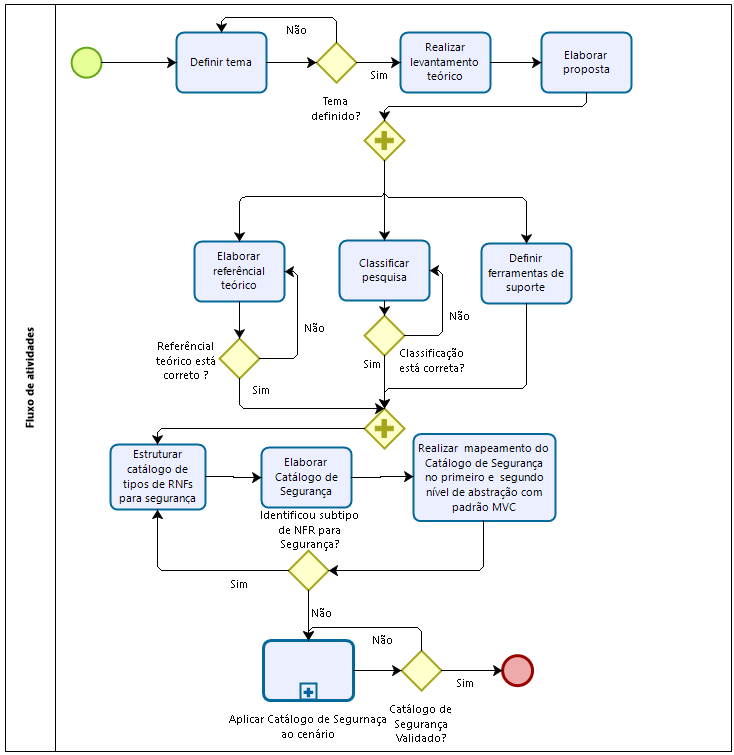
\includegraphics[keepaspectratio=true,scale=0.7]{figuras/fluxodeatividades.PNG}
	\caption{Atividades realizadas.}
	\label{fluxoDeExecuçãoTCC}
\end{figure}

Segue abaixo a descrição das atividades:

\begin{itemize}
	\item \textbf{Definir tema}: em conjunto com os professores orientadores dessa monografia, essa atividade teve como principal objetivo o refinamento sobre os conceitos teóricos referentes à área de interesse do autor;
	
	\item \textbf{Realizar levantamento teórico}: com base nos resultados obtidos na execução da atividade anterior, iniciou-se o levantamento teórico, seguindo as orientações dos orientadores. Discutiu-se sobre os aspectos fundamentais do GORE, os \textit{frameworks} que se apoiam nos conceitos do GORE, os conceitos de Arquitetura de Software e os atributos de qualidade mais relevantes para o mercado e para a academia;
	
	\item \textbf{Elaborar proposta}: com o conhecimento das necessidades da área de atuação desse trabalho, iniciou-se a elaboração da proposta de pequisa, acordando que seria utilizado o NFR \textit{Framework}, bem como, que seria aplicado ao mercado, tomando Segurança como o principal atributo de qualidade;  
	
	\item \textbf{Elaborar referencial teórico}: foi realizada a redação dos conceitos teóricos a serem aplicados no desenvolvimento desse trabalho; 
	
	\item \textbf{Classificar pesquisa}: redação  da classificação da pesquisa em suas dimensões sendo especificada quanto (i) à abordagem, (ii) à natureza, (iii) aos objetivos, e (iv) aos procedimentos técnicos;
	
	\item \textbf{Definir ferramentas de suporte}: definição e descrição das ferramentas utilizadas no desenvolvimento desse trabalho;
	
	\item \textbf{Estruturar catálogo de tipos de RNFs para Segurança}: com base nos conceitos de Segurança apresentados por Lawrence Chung, Brian A. Nixon, Eric Yu e John Mylopoulos, no  livro: \textit{NON-FUNCTIONAL REQUIREMENTS
	IN SOFTWARE ENGINEERING}, iniciou-se a elaboraçao  do catálogo de tipos de RNFs para Segurança, expandindo o catálogo com base em definições de subtipos de RNFs;
	
	\item \textbf{Elaborar Catálogo de Segurança}: a partir do Catálogo de Segurança, iniciou-se o processo de identificação das metas flexíveis que podem ser satisfeitas, orientando-se também pelo livro supracitado;
	
	\item \textbf{Realizar mapeamento do Catálogo de Segurança no primeiro e segundo nível de abstração com o padrão MVC}: iniciou-se a comparação das metas flexíveis que possuíam relação com o Padrão Arquitetural MVC e gerariam impactos positivos ou negativos na Segurança dos dados e da arquitetura. Durante a execução dessa atividade caso ocorresse a identificação de outro subtipo para Segurança à atividade, “Estruturar catálogo de tipos para Segurança” era realizada novamente e consequentemente as atividades seguintes de acordo com a Figura \ref{fluxoDeExecuçãoTCC}, e
	
	\item \textbf{Aplicar Catálogo de Segurança ao cenário}: essa atividade respeitou o processo de desenvolvimento de software descrito na seção \ref{sec:metodologiaDeDesenvolvimentoDeSoftware}
\end{itemize}

\subsection{Fluxo de Atividades do TCC2}

Este processo tem como principal objetivo a validação do catálogo proposto, através do desenvolvimento de uma aplicação de software. 

\begin{figure}[h!]
	\centering
	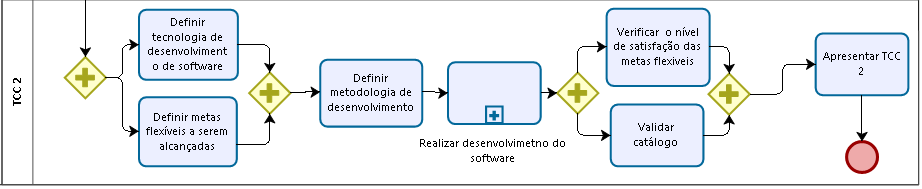
\includegraphics[keepaspectratio=true,scale=0.7]{figuras/PDM-TCC2.PNG}
	\caption{Atividades a serem realizadas no TCC2.}
	\label{PDM-TCC2}
\end{figure}

As atividades são:

\begin{itemize}
		
	\item \textbf{Definir metas flexíveis a serem alcançadas}: Definir as metas flexíveis a serem alcançadas de acordo com o cenário exemplo do software a ser desenvolvido.  
	
	\item \textbf{Macro atividade: Realizar desenvolvimento do software}: Realizar as etapas de desenvolvimento de acordo com a metodologia selecionada.
	
	\item \textbf{Verificar o nível de satisfação das metas flexíveis}: Verificar se as metas flexíveis foram alcançadas após o desenvolvimento do software.
	
	\item \textbf{Coletar as primeiras impressões da aplicação do catálogo}: Validar o catálogo de segurança porposto no TCC1 de acordo com o cenário especificado. 
	
	\item \textbf{Apresentar TCC 2}: Apresentar TCC 2 para a banca.
\end{itemize}

\subsection{Cronograma das Atividades}

O cronograma apresentado no Tabela \ref{cronograma-tcc1}, organizado em meses,  procura expor como se deu a execução das atividades do TCC1. 

Observa-se que foram utilizados, além do prazo base, os meses de Janeiro e Fevereiro. Isso ocorreu para um melhor aprofundamento do tema, o qual demandou a leitura de vários materiais bibliográficos. Adicionalmente, as notações envolvidas nessa pesquisa são complexas, necessitando de um cuidado maior na escrita, facilitando o entendimento por parte dos interessados.

\begin{table}[h!]
	\centering
	\caption{Cronograma das atividades para desenvolvimento do TCC1.}
	\label{cronograma-tcc1}
	\begin{tabular}{@{}lccccccc@{}}
		\hline
		\textbf{Atividade} & \multicolumn{1}{l}{\textbf{Ago}} & \multicolumn{1}{l}{\textbf{Set}} & \multicolumn{1}{l}{\textbf{Out}} & \multicolumn{1}{l}{\textbf{Nov}} & \multicolumn{1}{l}{\textbf{Dez}} & \multicolumn{1}{l}{\textbf{Jan}} & \multicolumn{1}{l}{\textbf{Fev}} \\ \hline
		Definir tema & \textbf{x} & \textbf{} & \textbf{} & \textbf{} & \textbf{} & \textbf{} & \textbf{} \\ \hline
		Realizar levantamento teórico & \textbf{x} & \textbf{x} & \textbf{} & \textbf{} & \textbf{} & \textbf{} & \textbf{} \\ \hline
		Elaborar proposta & \textbf{x} & \textbf{x} & \textbf{x} & \textbf{} & \textbf{} & \textbf{} & \textbf{} \\ \hline
		Elaborar referencial teórico & \textbf{} & \textbf{} & \textbf{x} & \textbf{x} & \textbf{x} & \textbf{} & \textbf{} \\ \hline
		Classificar pesquisa & \textbf{} & \textbf{} & \textbf{x} & \textbf{x} & \textbf{x} & \textbf{} & \textbf{} \\ \hline
		Definir ferramentas de suporte & \textbf{} & \textbf{} & \textbf{x} & \textbf{x} & \textbf{x} & \textbf{} & \textbf{} \\ \hline
		\begin{tabular}[c]{@{}l@{}}Estruturar catálogo de tipos \\ para segurança\end{tabular} & \textbf{} & \textbf{} & \textbf{} & \textbf{} & \textbf{x} & \textbf{x} & \textbf{} \\ \hline
		Elaborar SIG & \textbf{} & \textbf{} & \textbf{} & \textbf{} & \textbf{x} & \textbf{x} & \textbf{} \\ \hline
		\begin{tabular}[c]{@{}l@{}}Realizar mapeamento entre metas\\ flexíveis e o padrão MVC\end{tabular} & \textbf{} & \textbf{} & \textbf{} & \textbf{} & \textbf{} & \textbf{x} & \textbf{x} \\ \hline
		\begin{tabular}[c]{@{}l@{}}Definir metodologia de\\ desenvolvimento de software MVC\end{tabular} & \textbf{} & \textbf{} & \textbf{} & \textbf{} & \textbf{} & \textbf{x} & \textbf{x} \\ \hline
		\begin{tabular}[c]{@{}l@{}}Definir tecnologia de desenvolvimento\\ de software\end{tabular} & \textbf{} & \textbf{} & \textbf{} & \textbf{} & \textbf{} & \textbf{x} & \textbf{x} \\ \hline
		Apresentar TCC1 & \textbf{} & \textbf{} & \textbf{} & \textbf{} & \textbf{} & \textbf{} & \textbf{x} \\ \hline
	\end{tabular}
\end{table}

Na Tabela, é apresentado um planejamento para execução das atividades referentes ao TCC2. Trata-se de uma previsão, podendo ocorrer pequenos ajustes ao longo da realização do trabalho.

\begin{table}[h!]
	\centering
	\caption{Cronograma das atividades para desenvolvimento do TCC2.}
	\label{cronograma-tcc2}
	\begin{tabular}{@{}lccccc@{}}
		\hline
		\textbf{Atividade} & \multicolumn{1}{l}{\textbf{Mar}} & \multicolumn{1}{l}{\textbf{Abr}} & \multicolumn{1}{l}{\textbf{Mai}} & \multicolumn{1}{l}{\textbf{Jun}} & \multicolumn{1}{l}{\textbf{Jul}} \\ \hline
		Definir metas flexíveis a serem alcançadas & \textbf{x} & \textbf{} & \textbf{} & \textbf{} & \textbf{} \\ \hline
		Realizar desenvolvimento do software & \textbf{x} & \textbf{x} & \textbf{x} & \textbf{x} & \textbf{} \\ \hline
		\begin{tabular}[c]{@{}l@{}}Verificar o nível de satisfação das metas\\ flexíveis\end{tabular} & \textbf{} & \textbf{} & \textbf{x} & \textbf{x} & \textbf{} \\ \hline
		Coletar as primeiras impressões da \\ aplicação do catálogo & \textbf{} & \textbf{} & \textbf{} & \textbf{x} & \textbf{} \\ \hline
		Apresentar TCC 2 & \textbf{} & \textbf{} & \textbf{} & \textbf{x} & \textbf{} \\ \hline
	\end{tabular}
\end{table} 

\section{Resumo do Capítulo}

Neste capitulo, foi detalhada a classificação da pesquisa de acordo com seus tipos, como sendo a (i) abordagem de pesquisa, se tratando de uma pesquisa híbrida, a (ii) Natureza de pesquisa, caraterizada como uma pesquisa aplicada, o (ii) objetivo de pesquisa, caracterizado como uma pesquisa explicativa, e os (iv) procedimentos técnicos de pesquisa, caracterizados como uma pesquisa bibliográfica e a pesquisa ação. Tem-se ainda a adaptação do Scrum como método de desenvolvimento de software e o Kanban para acompanhamento visual do andamento da implementação das funcionalidades da aplicação web.

Adicionalmente, procurou-se detalhar ambos os fluxos de atividades e cronogramas para o pleno desenvolvimento do TCC1 e TCC2, respectivamente.

